\chapter{Curvature in MRMW}
\label{chapter-9-curvature}

\subsection{\textbf{Why some systems feel smooth, and others feel like broken glass.}}

In the daily practice of ordinary programming, the experience of building, debugging, refactoring, or optimizing a system is rarely a purely intellectual exercise. It is fundamentally, and often confusingly, emotional. We do not simply interact with logic; we interact with a landscape that pushes back.

Some systems feel distinctively friendly, welcoming changes with open arms. Others feel hostile, actively resisting every attempt at improvement. There are codebases that feel predictable, where effect follows cause in a straight line, and there are those that feel like trying to juggle glass cats in the middle of a hurricane.

When engineers describe these environments, they rarely reach for formal mathematics. Instead, they use tactile, visceral adjectives. They call a codebase "brittle" when it breaks under slight pressure, or "rigid" when it refuses to bend. They praise "elegant" solutions and curse "spaghetti" logic. They describe legacy systems as "hellish" or "fragile," while modern, well-tuned architectures are lauded as "robust" or "forgiving."

For decades, these descriptions have been treated as "vibes"---purely psychological reactions to messy code, devoid of rigorous mathematical backing.

\textbf{Until now.}

In a universe defined by Recursive Metagraphs and Double-Pushout (RMG+DPO) rewriting, these feelings are not merely psychological projections. They are detecting actual geometric properties of the underlying system. They stem from \textbf{geometry}---specifically, from \textbf{rulial curvature}.

This chapter is about exposing that invisible shape. We will explore why curvature exists, what it implies for the computational difficulty of a problem, and how it dramatically impacts the engineering experience. We will discover why some computational worlds are smooth planes while others are jagged, treacherous cliffs. We will see why, in high-curvature systems, small changes matter an extraordinary amount, making optimization feel like fighting gravity and debugging feel like climbing out of a deep pit.

Curvature is the invisible shape of your universe. It is time to make it visible.

---

\section{\textbf{9.1 --- What Curvature Means (Without Physics)}}

Before we descend into the mechanics, we must establish a crucial boundary to prevent conceptual baggage from muddying the waters.

\begin{quote}
\itshape
\textbf{\textit{This is NOT physical curvature.}}
\end{quote}

We are not discussing spacetime, general relativity, quantum gravity, or Einstein's field equations. We are not engaging in metaphysics. We are discussing \textit{computational curvature}, a precise measure of structural divergence.

In the context of MRMW, curvature is defined as:

\begin{quote}
\itshape
\textbf{The rate at which Rulial Distance expands as you move away from a given worldline.}
\end{quote}

Consider two almost identical states of a system. If you apply a sequence of valid rewrites to both, do they stay relatively similar, or do they diverge into completely unrecognizable structures?

If every small change to the graph produces only small, localized structural differences, we exist in a region of \textbf{low curvature}. The space is flat and predictable. However, if a minute change in the initial conditions or a single divergent rule application "blows up" into massive, systemic structural differences down the line, we are trapped in a region of \textbf{high curvature}.

Curvature is the sensitivity of a system to small transformations. It answers the fundamental question of stability: \textbf{How hard is it to stay near your intended worldline?}

This is the missing theoretical link behind every frustrated conversation engineers have ever had about "complexity," "technical debt," or "brittleness." We are finally describing these phenomena formally.

\begin{figure}[h]
\centering
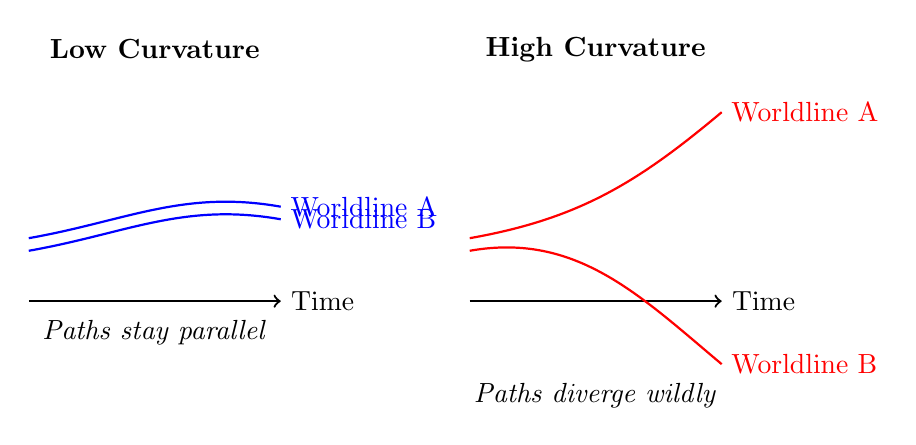
\begin{tikzpicture}[scale=0.8]
    % Low Curvature
    \node at (2, 4) {\textbf{Low Curvature}};
    \draw[thick, ->] (0,0) -- (4,0) node[right] {Time};
    \draw[blue, thick] (0,1) to[out=10, in=170] (4,1.5);
    \draw[blue, thick] (0,0.8) to[out=10, in=170] (4,1.3);
    \node[right, blue] at (4,1.5) {Worldline A};
    \node[right, blue] at (4,1.3) {Worldline B};
    \node at (2, -0.5) {\textit{Paths stay parallel}};

    % High Curvature
    \begin{scope}[shift={(7,0)}]
        \node at (2, 4) {\textbf{High Curvature}};
        \draw[thick, ->] (0,0) -- (4,0) node[right] {Time};
        \draw[red, thick] (0,1) to[out=10, in=220] (4,3);
        \draw[red, thick] (0,0.8) to[out=10, in=140] (4,-1);
        \node[right, red] at (4,3) {Worldline A};
        \node[right, red] at (4,-1) {Worldline B};
        \node at (2, -1.5) {\textit{Paths diverge wildly}};
    \end{scope}
\end{tikzpicture}
\caption{Visualizing Rulial Curvature: In low curvature (left), small state changes result in similar futures. In high curvature (right), a small state change results in radically different futures.}
\end{figure}

---

\section{\textbf{9.2 --- Low Curvature: Smooth, Friendly, Forgiving Systems}}

When a system exhibits low curvature, it possesses a specific kind of geometric stability. In these regions, nearby "Time Cubes" overlap significantly. Many different rewrite sequences lead to structurally similar worlds, meaning that the exact order of operations often matters less than the aggregate result. Legal transformations cascade gently through the graph, and structural invariants work in harmony with the developer rather than fighting against them.

In a low-curvature universe, small divergences reconverge naturally. Optimization paths feel intuitive because the gradient is smooth; you can see the destination and walk toward it. Refactoring does not cause explosions, and debugging feels like walking downhill—gravity is on your side.

\subsection{\textbf{The universe around your worldline is smooth.}}

If you take a step left or right in the state space, you remain in the same neighborhood. This geometric smoothness is the defining characteristic of many technologies that engineers inherently love.

Consider systems like Entity Component Systems (ECS) in game development, where data is laid out linearly and dependencies are minimized. Consider well-designed Functional Reactive Programming (FRP) architectures, or languages with strong normalization properties. Pure functional pipelines, linear algebra libraries, and declarative build systems all share this property. Even SQL query optimizers rely on this; they assume that transforming the query graph (the plan) won't result in a wildly different output, just a more efficient path to the same data.

In these systems, the "cone" of future possibilities points downhill. You can physically feel the geodesic pulling you toward the correct solution.

---

\section{\textbf{9.3 --- High Curvature: Jagged, Brittle, Spiky Universes}}

Conversely, a system dominated by high curvature is a hostile environment. Here, the butterfly effect is not a metaphor; it is the daily operational reality. Small changes produce massive, catastrophic divergences.

In these jagged spaces, many DPO rules block each other. Applying Rule A invalidates the preconditions for Rule B, forcing the system into a corner. Invariants fight one another, creating tension where any move breaks a rule. The Time Cube becomes dangerously narrow; the number of legal next steps vanishes abruptly, leaving the system stalled or crashed.

Adjacent universes in high-curvature space behave wildly differently. A single boolean flag change might alter the entire control flow of the application. Debugging feels like climbing uphill in loose gravel, where every step slides you backward. Optimization feels like bushwhacking through a dense jungle with no line of sight. Refactoring feels less like architecture and more like disarming a live bomb.

We see this geometry manifest in tangled imperative control flow, ad-hoc stateful systems, and the nightmare of circular dependencies. It appears in inconsistent database schemas, legacy codebases that mix four different programming paradigms, and game engines built over twenty years of crunch time. It is the hallmark of unbounded mutation and "stringly-typed" logic.

These systems have \textit{spikes} in the rulial manifold. You move one tick sideways, and you fall into a pit. Engineers call these systems "cursed." Now, you understand that "cursed" is simply a colloquialism for "geometrically unstable."

---

\section{\textbf{9.4 --- How Curvature Shapes Worldlines}}

Curvature is not just a theoretical metric; it fundamentally dictates the mechanics of engineering work across several axes.

\subsection{\textbf{Debugging}}
In a low-curvature environment, mistakes stay near the intended worldline. If you introduce a bug, the system state is only slightly perturbed, making it easy to trace the error back to its source. In high curvature, a tiny divergence—an off-by-one error or a race condition—can transport the universe into an entirely alien region of the state space. You aren't just looking for a bug; you are trying to understand how you ended up on a different planet.

\subsection{\textbf{Optimization}}
Optimization is the act of straightening the worldline, finding the geodesic. In low-curvature space, straightening the path is intuitive because the topology is simple. In high-curvature space, the "shortest path" might require traversing a complex labyrinth. The "wrong door" doesn't just slow you down; it leads to a dead end.

\subsection{\textbf{Refactoring}}
Refactoring is essentially a homotopy—a continuous deformation of the code structure. Low curvature ensures that safe transformations abound; you can mold the clay without it cracking. High curvature means the material is brittle; invariants snap under the pressure of minor edits, and the system shatters rather than reshapes.

\subsection{\textbf{Design}}
Design is the act of setting the curvature. In good design, rules reinforce each other, smoothing out the manifold. In poor design, rules cross-cut and fight at the boundaries, creating ridges and spikes in the geometry.

Ultimately, curvature is the difference between a system that feels like it \textit{wants} to work, and a system that feels like it \textit{wants} to die.

---

\section{\textbf{9.5 --- Curvature and the Time Cube}}

Recall the Time Cube: the localized cone of legal next futures available to a system at any given moment. Curvature dramatically alters the behavior of this cone.

\begin{figure}[h]
\centering
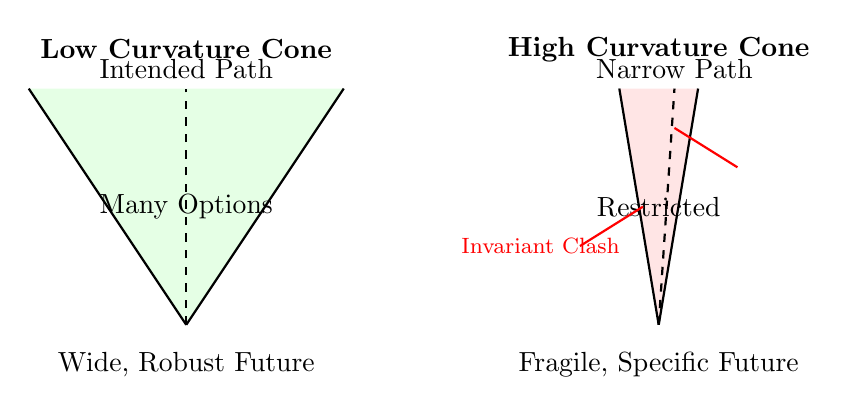
\begin{tikzpicture}
    % Wide Cone (Low Curvature)
    \node at (0, 3.5) {\textbf{Low Curvature Cone}};
    \fill[green!20, opacity=0.5] (0,0) -- (2,3) -- (-2,3) -- cycle;
    \draw[thick] (0,0) -- (2,3);
    \draw[thick] (0,0) -- (-2,3);
    \draw[thick, dashed] (0,0) -- (0,3) node[above] {Intended Path};
    \node at (0, 1.5) {Many Options};
    \node at (0, -0.5) {Wide, Robust Future};

    % Narrow Cone (High Curvature)
    \begin{scope}[shift={(6,0)}]
        \node at (0, 3.5) {\textbf{High Curvature Cone}};
        \fill[red!20, opacity=0.5] (0,0) -- (0.5,3) -- (-0.5,3) -- cycle;
        \draw[thick] (0,0) -- (0.5,3);
        \draw[thick] (0,0) -- (-0.5,3);
        \draw[thick, dashed] (0,0) -- (0.2,3) node[above] {Narrow Path};
        \node at (0, 1.5) {Restricted};
        \node at (0, -0.5) {Fragile, Specific Future};
        
        % Spikes / Blockers
        \draw[thick, red] (-1, 1) -- (-0.2, 1.5);
        \draw[thick, red] (1, 2) -- (0.2, 2.5);
        \node[red, font=\footnotesize] at (-1.5, 1) {Invariant Clash};
    \end{scope}
\end{tikzpicture}
\caption{The Geometry of Options. Low curvature offers a wide cone of legal moves. High curvature offers a narrow path where deviation leads to failure.}
\end{figure}

In a \textbf{low curvature} region, the cone is wide. The options for the next computational step are plentiful. Nearby worlds are similar enough that choosing one path over another is rarely fatal. Turning the system "sideways" feels natural.

In a \textbf{high curvature} region, the cone is terrifyingly narrow. The options are few. Nearby worlds are not similar; they are jaggedly disjoint. Turning at all feels catastrophic because the walls of the cone are closing in. This describes exactly why technical debt feels "heavy." It is not a psychological weight; it is the geometric constriction of your future options. You are operating in a region where the geometry itself resists change.

---

\section{\textbf{9.6 --- Curvature Across Multiple Models (MR Axis)}}

This is where the concept of curvature spills over into the broader \textbf{MRMW} framework. Changing the rules (the MR axis) changes the shape of the manifold itself.

A slight tweak to your DPO invariants—the fundamental rules of your rewrite system—might flatten the curvature, making everything smoother and opening up the Time Cone. Alternatively, a careless rule change might increase the jaggedness, introducing new spikes into the terrain.

This realization explains why \textbf{language design} and \textbf{system architecture} are such high-stakes disciplines. When you design a language or an API, you are not merely deciding what computation \textit{does}. You are deciding what \textbf{curvature} that computation will live inside.

Domain Specific Languages (DSLs) are tools to flatten curvature within a specific problem space. Type systems are guardrails that constrain curvature, preventing the graph from folding into invalid shapes. Compiler passes are automated mechanisms to straighten worldlines.

When you engage in these activities, you are not writing code. You are \textbf{curating geometry.}

---

\section{\textbf{9.7 --- Curvature Is Why NP Sometimes Collapses Locally}}

This serves as the primer for the revelations of Chapter 10. We have established that high curvature makes traversal difficult, but what happens in regions of extreme low curvature?

In these smooth, highly structured regions, problems that are theoretically exponential (NP-hard) in the general case explode significantly less. Why does this happen?

It happens because the rulial manifold contains structural shortcuts. These are legal rewrites that effectively "fold space," shortening the path between the start state and the solution state inside the Time Cube. This phenomenon is known as \textbf{local NP collapse}.

To be absolutely clear:
This is \textbf{\textit{not}} global. We are not claiming P = NP.
This is \textbf{\textit{not}} magical thinking.
This is \textbf{\textit{not}} anti-Turing or quantum woo.

It is simply the realization that:

\begin{quote}
\itshape
\textbf{When structure is strong enough, search becomes navigation.}
\end{quote}

In a chaotic graph, you must search every path. In a structured, low-curvature graph, you can navigate by landmarks. Chapter 10 is where we drop this hammer.

---

\section*{FOR THE NERDS }

\subsection{Curvature $\approx$ Sensitivity of the Rulial Metric Tensor}

\textit{(A brief aside for those craving the formal mechanics, though we do not need tensors to use the intuition.)}

Formally, \textbf{Curvature in Rulial Space can be approximated as the second derivative of Rulial Distance with respect to local rewrites.}

If $D(G_1, G_2)$ is the edit distance between two graphs, curvature measures how $\frac{d}{dt} D(G_1(t), G_2(t))$ changes as the graphs evolve under the rule set $\mathcal{R}$.

However, you do not need differential geometry to apply this concept to software engineering. You simply need to internalize the correspondence:

\begin{itemize}
\item \textbf{High Curvature} = Sensitive, chaotic regions where $\Delta_{output} \gg \Delta_{input}$.
\item \textbf{Low Curvature} = Stable, linear regions where $\Delta_{output} \approx \Delta_{input}$.
\item \textbf{Origin} = Curvature is not inherent to the data; it emerges from the interaction between the data structure and the transition rules.
\end{itemize}

\textit{(End sidebar.)}

---

\section{\textbf{9.8 --- Transition: From Curvature to Collapse}}

Now that we have successfully visualized curvature, we are equipped to tackle one of the most fascinating consequences of this geometry. We are approaching the concept of regions where computation becomes exponentially easier—not because the computer is faster, but because the worldline has many shortcuts.

This isn't about breaking the laws of complexity classes. It is about recognizing that in highly structured manifolds, search algorithms collapse under the weight of favorable geometry.

Chapter 10 is the "oh shit" moment of Part III.
